% Reports (up to ~2500 words including references, notes and captions–corresponds to ~3
% printed pages in the journal) present important new research results of broad
% significance. Reports should include an abstract, an introductory paragraph, up to
% four figures or tables, and about 30 references. Materials and Methods should be
% included in supplementary materials, which should also include information needed to
% support the paper's conclusions.

% Main Text is not divided into sub-headings for Reports.

% The manuscript should start with a brief introduction describing the paper’s
% significance. The introduction should provide sufficient background information to
% make the article intelligible to readers in other disciplines, and sufficient context
% that the significance of the experimental findings is clear.

Since early 2020, the CoViD-19 pandemic has presented an enormous challenge to humanity
on many dimensions. The development of highly effective vaccines holds the promise of
containment in the medium term. However, most countries find themselves many
months---and often years---away from reaching vaccination-induced herd immunity
\citep{Swaminathan2021}.\comment[id=K]{WHO Press Conference saying we won't reach herd
immunity in 2021}\comment[id=HM]{If we find a paper (s)he cites, would be even better}
In the meantime, it is of utmost importance to employ an effective mix of strategies for
containing the virus. The most frequent initial response was a set of non-pharmaceutical
interventions (NPIs) to reduce contacts between individuals. While this has allowed some
countries to sustain equilibria with very low infection numbers\footnote{See
    \citet{Contreras2021} for a theoretical equilibrium at low case numbers which is
    sustained with test-trace-and-isolate policies.}, most have seen large fluctuations of
infection rates. Containment measures have become increasingly diverse and now include
testing, more nuanced NPIs, and contact tracing. Neither these policies' effect nor the
influence of seasonal patterns or more infectious virus strains are well understood in
quantitative terms. This paper develops a model incorporating all these factors. The
framework allows to combine a wide variety of data in a timely fashion, making it useful
to predict the effects of various interventions. We apply the model to Germany and show
that rapid testing had the largest impact on the reduction in infections by almost 80\%
during the month of May 2021. We conclude that rapid tests have a large role to play at
least as long as vaccinations have not been offered to an entire population.

At the core of our agent-based model are physical contacts between heterogeneous agents
(Figure~\ref{fig:broad_model_description}).\footnote{We provide a detailed comparison to
    other approaches in \ref{sec:literature_review}. The model most closely related to ours
    is described in \citet{Hinch2020}.} Each contact between an infectious individual and
somebody susceptible to the disease bears the risk of transmitting the virus. Contacts
occur in the household, at work, at school, or in other settings (leisure activities,
grocery shopping, medical appointments, etc.). Some contacts recur regularly, others
occur at random. Random contacts are typically assortative in age and geographical
location. Empirical applications can take the population structure from census data and
the types and frequency of contacts from diary data measuring contacts before the
pandemic \citep[e.g.][]{Mossong2008}.\footnote{\citet{Hoang2019} provide access to
    multiple data sets on contact types and frequencies at
    \url{http://www.socialcontactdata.org/} covering countries from all continents except
    North America and Australia.} The dimensions are chosen so that the most common NPIs can
be modeled in great detail by reducing the number of contacts in a particular setting or
the risk of transmitting the disease for a type of contact. For example, a mandate to
work from home will reduce the number of work contacts to zero for a fraction of the
working population. Schools and daycare can be closed entirely, operate at reduced
capacity---including an alternating schedule---,or implement mitigation measures like
masking requirements or air filters \citep{Lessler2021}. Curfews may reduce the number
of contacts in non-work/non-school settings. In any setting, measures like masking
requirements would reduce the probability of infection associated with a contact.

\begin{figure}
    \centering

    \begin{subfigure}[b]{0.425\textwidth}
        \centering
        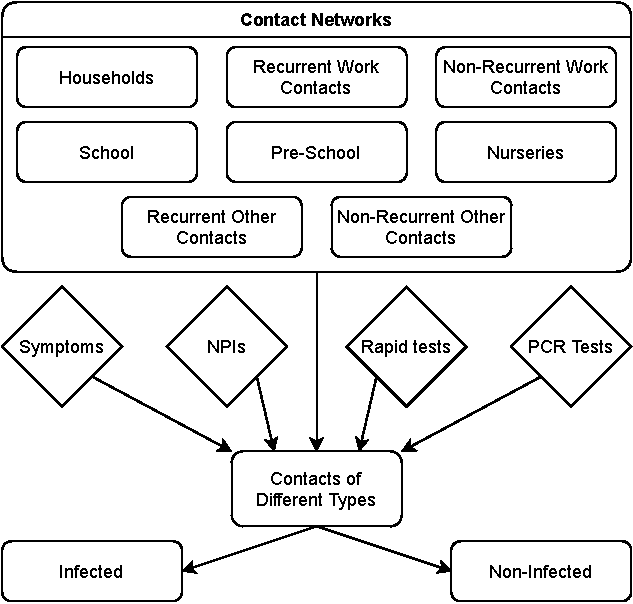
\includegraphics[width=\textwidth]{../figures/model-graph-top-left}
        \caption{{Model description}}
        \label{fig:broad_model_description}
    \end{subfigure}
    \hfill
    \begin{subfigure}[b]{0.425\textwidth}
        \centering
        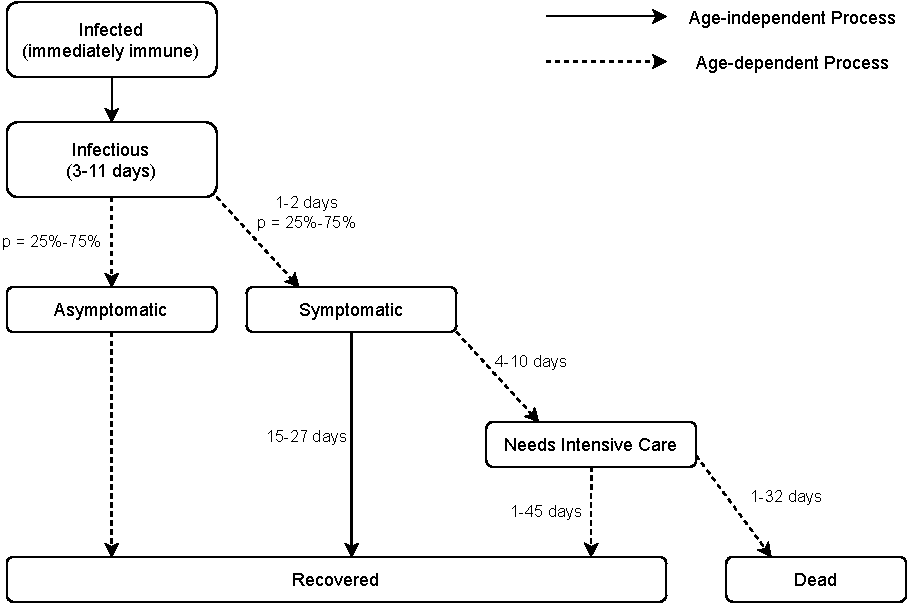
\includegraphics[width=\textwidth]{../figures/model-graph-top-right}
        \vskip4ex


        \caption{Disease progression}
        \label{fig:disease_progression}
    \end{subfigure}
    \vskip3ex
    \begin{subfigure}[b]{0.425\textwidth}
        \centering

        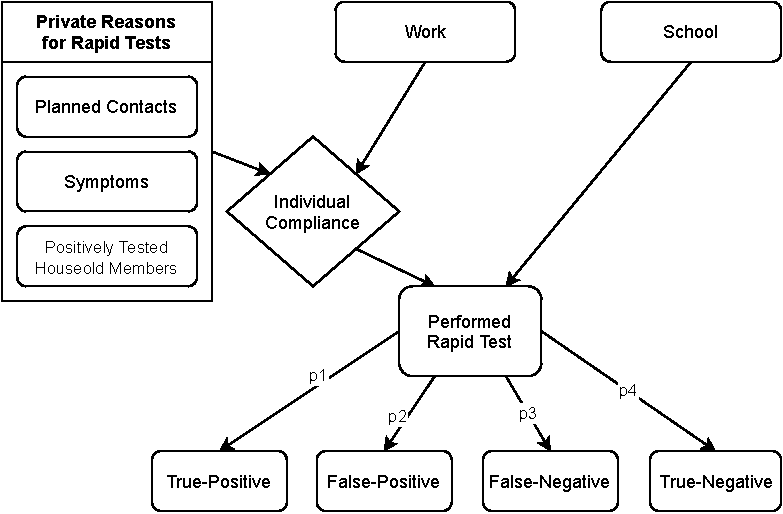
\includegraphics[width=\textwidth]{../figures/model-graph-bottom-left}
        \caption{{Model for antigen tests}}
        \label{fig:antigen_tests}
    \end{subfigure}
    \hfill
    \begin{subfigure}[b]{0.425\textwidth}
        \centering
        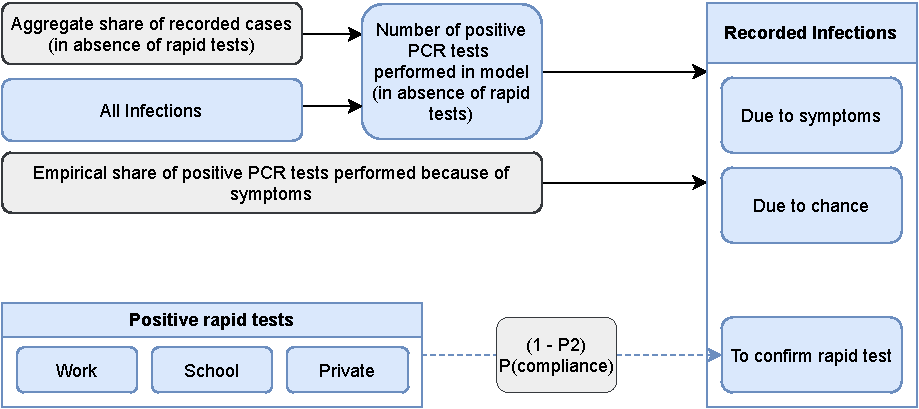
\includegraphics[width=\textwidth]{../figures/model-graph-bottom-right}
        \caption{{Model for undetected cases}}
        \label{fig:model_for_official_cases}
    \end{subfigure}

    \caption{Model description}
    \label{fig:model-description}

    \floatfoot{\noindent Note: ...}
\end{figure}

In our model, susceptibility to contracting the SARS-CoV-2 virus is dependent on age. A
possible infection progresses as shown in Figure~\ref{fig:disease_progression}. We
differentiate between an initial period of infection without being infectious or showing
symptoms, being infectious (presymptomatic or asymptomatic), showing symptoms, requiring
intensive care, and recovery or death as for example also modeled in \cite{Grimm2021}.
The probabilities of transitioning between these states depend on age; their duration is
random within intervals calibrated to medical literature (for a detailed description see
Section~\ref{sec:medical_params}). Conditional on the type of contact, infectiousness is
independent of age \citep{Jones2021}.

The model includes several other features, which are crucial to describe the evolution
of the pandemic in 2020-2021. New virus strains with different profiles regarding
infectiousness can be introduced. Agents may receive a vaccination. With a probability
of 75\% \citep{Hunter2021}, vaccinated agents become immune and they do not transmit the
virus \citep{Petter2021, LevineTiefenbrun2021, Pritchard2021}.\comment[id=T]{Maybe add
that 35\% reach immunity after two weeks and 40\% after three weeks.}\footnote{75\% is
    lower than what is usually reported for after the second dose of the Biontech/Pfizer
    vaccine, which is most commonly used in Germany. We choose it because our model neither
    includes booster shots, nor does it allow vaccinated individuals who became immune to
    transmit the disease\citep{Petter2021, LevineTiefenbrun2021, Pritchard2021}. If
    anything, these assumptions would overstate the effect of vaccines for our study period.
    This would be different if a large fraction of vaccinated individuals had received a
    second dose already.} During the vaccine roll-out, priority may depend on age and
occupation.

We include two types of tests. Polymerase chain reaction (PCR) tests directly reveal
whether an individual is infected or not. PCR tests require some days to be processed
and there are always aggregate capacity constraints. In contrast, rapid antigen tests
yield immediate results. Specificity and sensitivity of these tests is set according to
data analyzed in \cite{Bruemmer2021, Smith2021}; sensitivity depends on the timing of
the test relative to the start of infectiousness. Figure~\ref{fig:antigen_tests} shows
our model for rapid test demand. Schools may require students to be tested regularly.
Rapid tests may be offered by employers for on-site workers. Individuals may demand
tests for private reasons, which include having plans to meet other people\footnote{A
    positive test will make them reduce their contacts; this is why tests impact the actual
    contacts in Figure~\ref{fig:model-description}.}, showing symptoms of CoViD-19, and
because a household member tested positively for the virus. We endow each agent with an
individual compliance parameter. This parameter determines whether she takes up rapid
tests offered by employers or follows up on private reasons. The thresholds are lower
for tests in a private setting than for tests at the workplace.\comment[id=HM]{True?
@Janos}

Modelling a population of agents according to actual demographic characteristics means
that we can use a wide array of data to identify and estimate the model's many
parameters.\footnote{See section S.XXX of the supplementary materials for an overview.}
Mobility data is used to model the reductions in work contacts. School and daycare
policies are incorporated directly from official directives. Infection rates by age and
geographical region are estimated to match to officially recorded numbers; so is the
prevalence of virus strains. The model yields total infections, but only a fraction of
those will be officially recorded. We model the fraction of known cases as depicted in
Figure~\ref{fig:model_for_official_cases}.\comment[id=HM]{Add a sentence.}
% \footnote{EQUATIONS FOR THE FOURTH PICTURE (find names!):

%     The probabilities for Figure~\subref{fig:model_for_official_cases} are the
%     following:

%     \begin{align*} x & = \frac{n\_newly\_infected \times share\_known\_cases \times
%         P(PCR | S)}{n\_symptomatic\_and\_untested}                    \\
%         y & = \frac{n\_newly\_infected \times share\_known\_cases \times P(PCR |
%         S)}{n\_asymptoptomatic\_and\_infected\_and\_untested} \\
%         z & = \frac{P(PCR | RT)}{survey} \end{align*} where untested means that
%     individuals are not waiting on the result of a previously administered rapid
%     test.} 
A further advantage is that the simulated data have a structure that resembles datasets
used for regression models, which allows additional plausibility checks by re-running
the same models on the model-generated data.\comment[id=HM]{Only keep if we actually do
something like that.}

We apply this model to Germany. In March and April 2020, the country broke the first
wave of the pandemic fairly quickly. Between May and mid-September, daily new infections
were below 20 per Million and day \citep{owidcoronavirus}. We model the period
mid-September 2020 to the end of May 2021. We pick the starting date for two reasons.
First, we do not include the first wave because the environment was very different
(e.g., aggregate PCR test capacity was much lower and we would require a very different
model for calculating the share of known cases). Second, a large fraction of cases
during summer of 2020 were traced to international travel
\citep{KochInstitut2021,Hodcroft2021} but the precise number is difficult to model.

Figure~\ref{fig:pandemic_drivers_model_fit} describes the evolution of the pandemic and
of its drivers. The black line in Figure~\ref{fig:aggregated_fit} shows officially
recorded cases; the black line in Figure~\ref{fig:stringency_index} the Oxford Response
Stringency Index \citep{Hale2020}, which tracks the tightness of non-pharmaceutical
interventions. We transform the index so that lower values represent higher levels of
restrictions. A value of zero means all measures incorporated in the index are turned
on. The value 1 represents the situation in mid-September, with restrictions on
gatherings and public events, masking requirements, but open schools and workplaces (the
raw value of the index at that point is 49.5). In the seven weeks between mid September
and early November, cases increased by a factor of 10. Restrictions were somewhat
tightened in mid-October and again in early November. New infections remained constant
throughout November, before rising again in December, which prompted the most stringent
lockdown to this date. Schools and daycare centers were closed again, so were
customer-facing businesses except for grocery and drug stores. From the peak of the
second wave just before Christmas until the trough in mid-February, newly detected cases
decreased by almost three quarters. The third wave in the spring of 2021 is associated
with the B.1.1.7 strain, which became dominant in March. See
Figure~\ref{fig:share_b117}. In early March, some NPIs were being relaxed; e.g.,
hairdressers and home improvement stores were allowed to open again to the public.


\begin{figure}[!tp]
    \centering

    \begin{subfigure}[b]{0.475\textwidth}
        \centering
        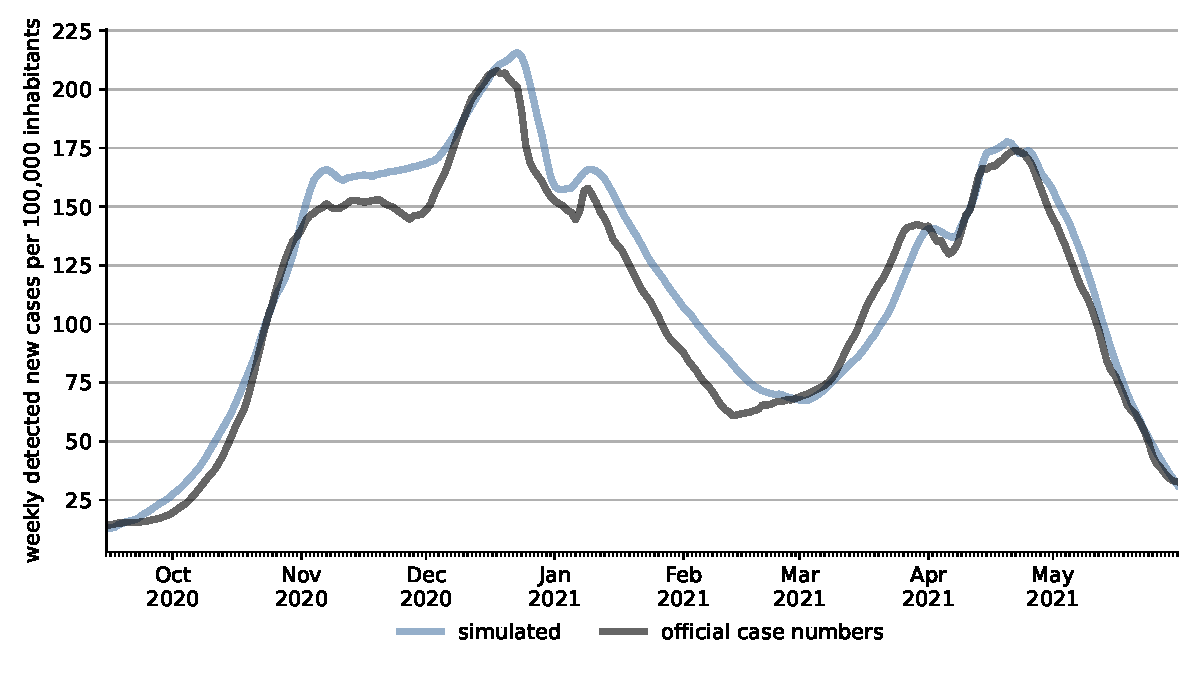
\includegraphics[width=\textwidth]{../figures/results/figures/scenario_comparisons/combined_fit/full_new_known_case}
        \caption{{Recorded cases: Empirical and simulated}}
        \label{fig:aggregated_fit}
    \end{subfigure}
    \hfill
    \begin{subfigure}[b]{0.475\textwidth}
        \centering
        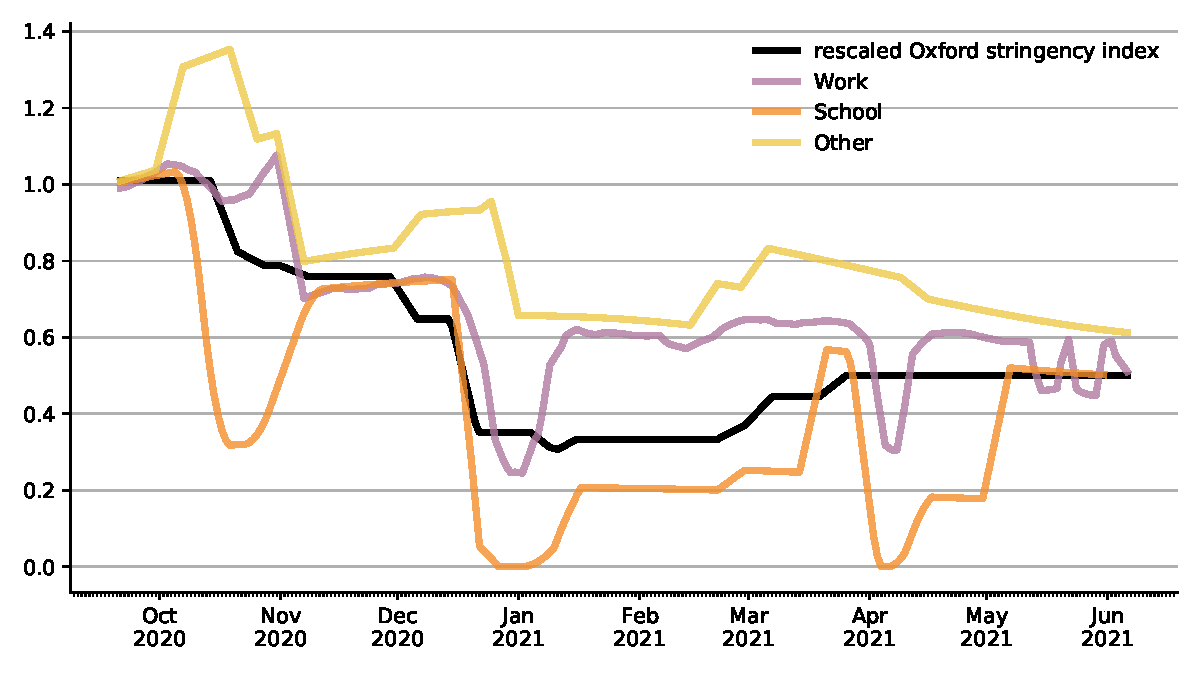
\includegraphics[width=\textwidth]{../figures/results/figures/data/stringency2_with_seasonality}

        \caption{{Stringency of NPIs and infectious contacts}}
        \label{fig:stringency_index}
    \end{subfigure}

    \vskip3ex

    \begin{subfigure}[b]{0.475\textwidth}
        \centering

        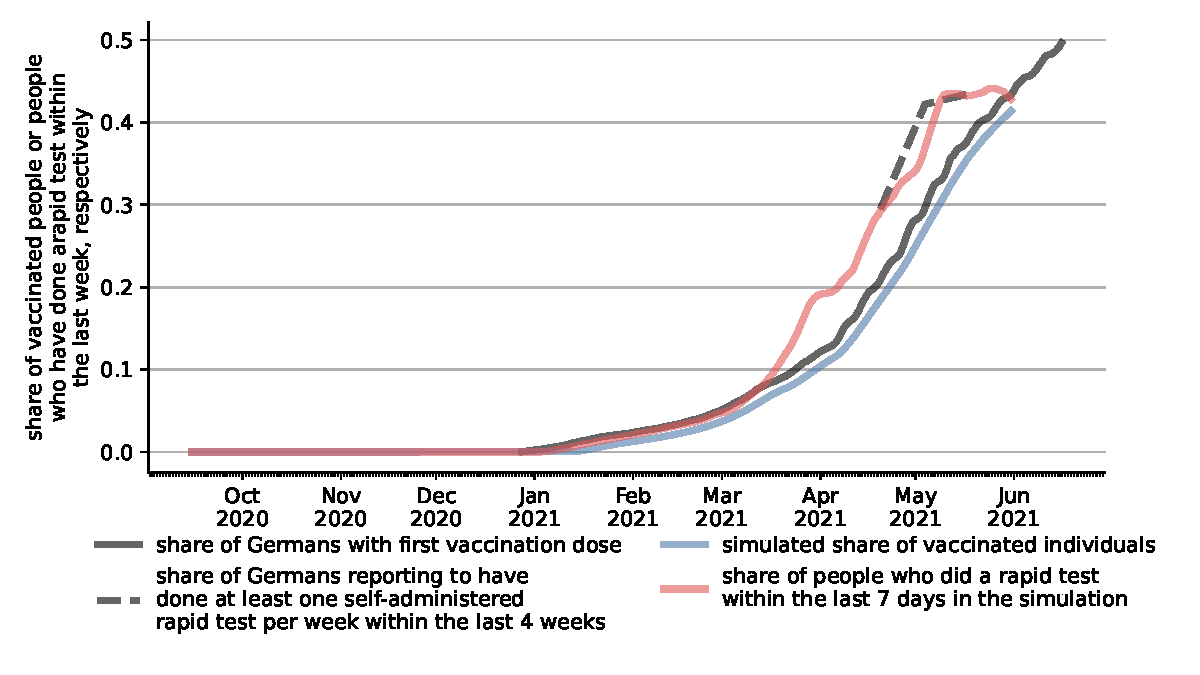
\includegraphics[width=\textwidth]{../figures/results/figures/scenario_comparisons/combined_fit/full_share_rapid_test_in_last_week_and_vaccinated}

        \caption{{Tests and vaccinations}}
        \label{fig:antigen_tests_vaccinations}
    \end{subfigure}
    \hfill
    \begin{subfigure}[b]{0.475\textwidth}
        \centering

        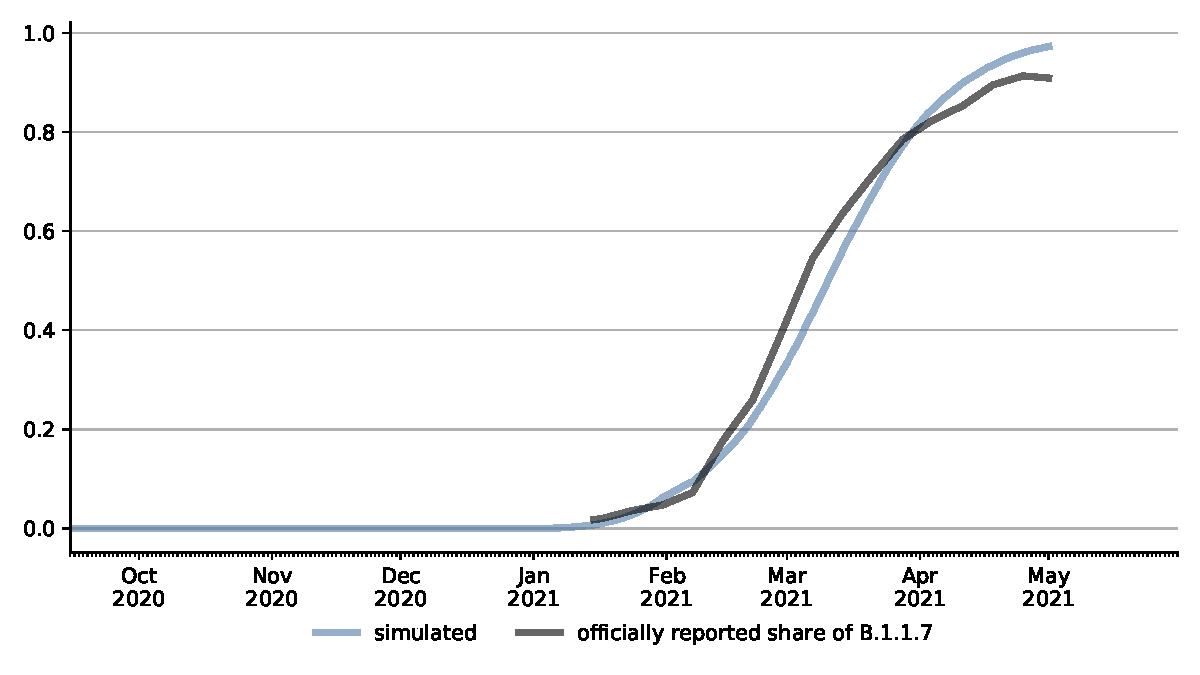
\includegraphics[width=\textwidth]{../figures/results/figures/scenario_comparisons/combined_fit/full_share_b117}

        \caption{Fraction of B.1.1.7 strain}
        \label{fig:share_b117}
    \end{subfigure}

    \caption{Evolution of the pandemic, its drivers, and model fit, September 2020 to May 2021}
    \label{fig:pandemic_drivers_model_fit}

    \floatfoot{\noindent Note: All aggregates; See S.XXX for statistics by age group and
        by geographical region. Also more disaggregated data.

        Sources: ...}

\end{figure}

By this time, the set of policy instruments had become much more diverse. Around the
turn of the year, the first people were vaccinated with a focus on older age groups and
medical personnel (Figure~\ref{fig:antigen_tests_vaccinations}. By the end of May, just
over 40\% had received at least one dose of a vaccine. Around the same time, rapid tests
started to replace PCR tests in many medical and nursing facilities. These had to be
administered by medical doctors or in pharmacies. At-home tests approved by authorities
became available in mid-March, rapid test centers were opened and one test per person
and week was made available free of charge. Depending on the state, customers were only
allowed to enter certain stores with a recent negative rapid test result. These
developments are characteristic of many countries: The initial focus on NPIs to slow the
spread of the disease has been accompanied by vaccines and a growing acceptance and use
of rapid tests. At broadly similar points in time, novel strains of the virus have
started to pose additional challenges.

Our model is able to track these developments very well. The blue line in
Figure~\ref{fig:aggregated_fit} shows our model's predictions are very close to
officially recorded cases in the aggregate. This is also true for infections by age and
geographical region, which are shown in the supplementary materials
(Figures~\ref{fig:age_group_fit} and \ref{fig:state_fit}, respectively). We can
disentangle various mechanisms due to the distinct temporal variation in the drivers of
the pandemic. Next to the stringency index, the three lines in
Figure~\ref{fig:stringency_index} summarize how contact reductions, increased hygiene
regulations, and seasonality evolved since early September for each of the three broad
contact networks. For example, a value of 0.75 for the work multiplier means that if the
environment was the same as in September (levels of infection rates, no rapid tests or
vaccinations, only the wildtype virus present), infections at the workplace would be
reduced by 25\%. This reduction is the product of the effect of contact reductions,
increased hygiene regulations, and seasonality. Along with the levels of infections,
these measures determine the spread of SARS-CoV-2 in 2020. See
Appendix~\comment[id=HM]{Reference} for separate plots of the three factors. Two aspects
are particularly interesting. First, all lines broadly follow the stringency index and
they would do so even more if we left out seasonality and school vacations (roughly the
last two weeks of October, two weeks each around Christmas and Easter, and some days in
late May). Second, the most stringent regulations are associated with the period of
strong decreases in new infection between late December 2020 and mid-February 2021. The
measures were not enough, however, to stop the B.1.1.7 variant from spreading in the
subsequent period. The steep drop in recorded cases during May 2021 is associated with
at least weekly rapid tests to around 42~percent of the population, a vaccination rate
that rose from 28\% to 43\%, and mostly seasonality impacting a fall in the relative
infectiousness of contacts outside of work and school.

Figure~\ref{fig:2021_scenarios_broad} consider the relative effects of rapid tests,
vaccinations, and of seasonality during 2021, assuming NPIs to have evolved the same way
as in the baseline scenario. Figure~\ref{fig:2021_scenarios_recorded} shows the model
fit (the blue line, same as in Figure~\ref{fig:aggregated_fit}), a scenario without any
of the three factors (red line), and three scenarios turning these factors off one by
one. Figure~\ref{fig:2021_scenarios_newly_infected} does the same for total infections
in the model. Figure~\ref{fig:2021_scenarios_decomposition} employs Shapley values to
decompose the difference in total infections between the scenario without any of the
three factors and our main specification.

\begin{figure}[!tp]
    \centering

    \begin{subfigure}[b]{0.475\textwidth}
        \centering
        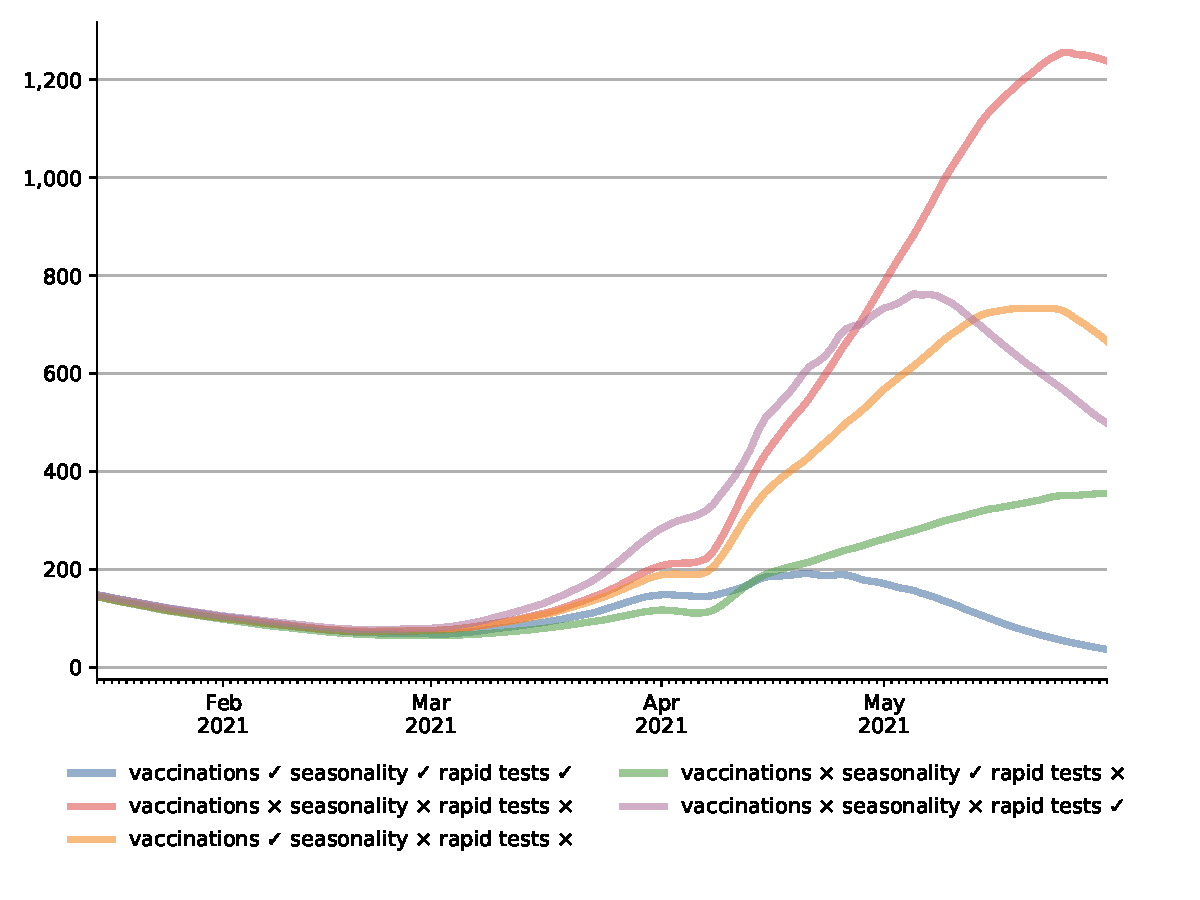
\includegraphics[width=\textwidth]{../figures/results/figures/scenario_comparisons/effect_of_channels_on_pessimistic_scenario/full_new_known_case}
        \caption{{Recorded cases: 2021 scenarios}}
        \label{fig:2021_scenarios_recorded}
    \end{subfigure}
    \hfill
    \begin{subfigure}[b]{0.475\textwidth}
        \centering
        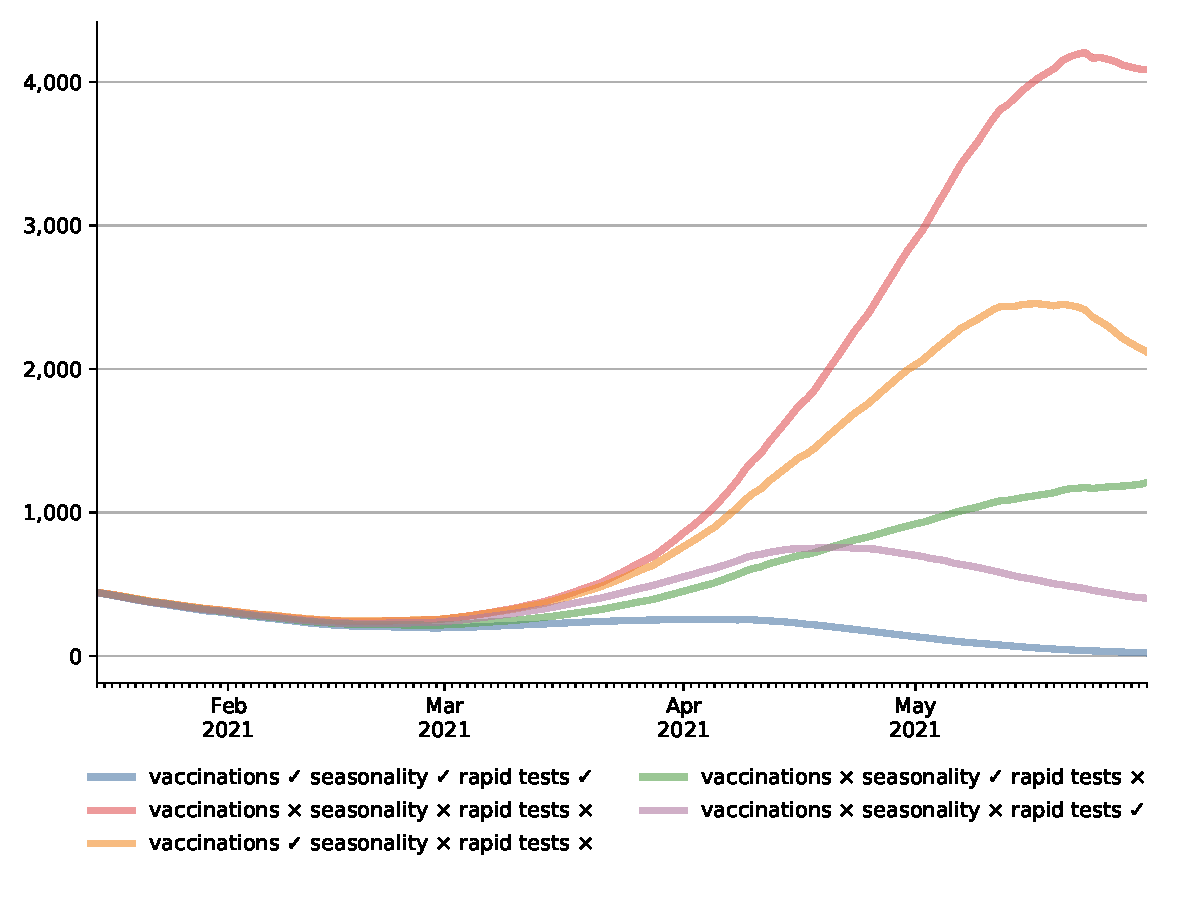
\includegraphics[width=\textwidth]{../figures/results/figures/scenario_comparisons/effect_of_channels_on_pessimistic_scenario/full_newly_infected}
        \caption{{Total cases: 2021 scenarios}}
        \label{fig:2021_scenarios_newly_infected}
    \end{subfigure}

    \begin{subfigure}[b]{0.475\textwidth}
        \centering
        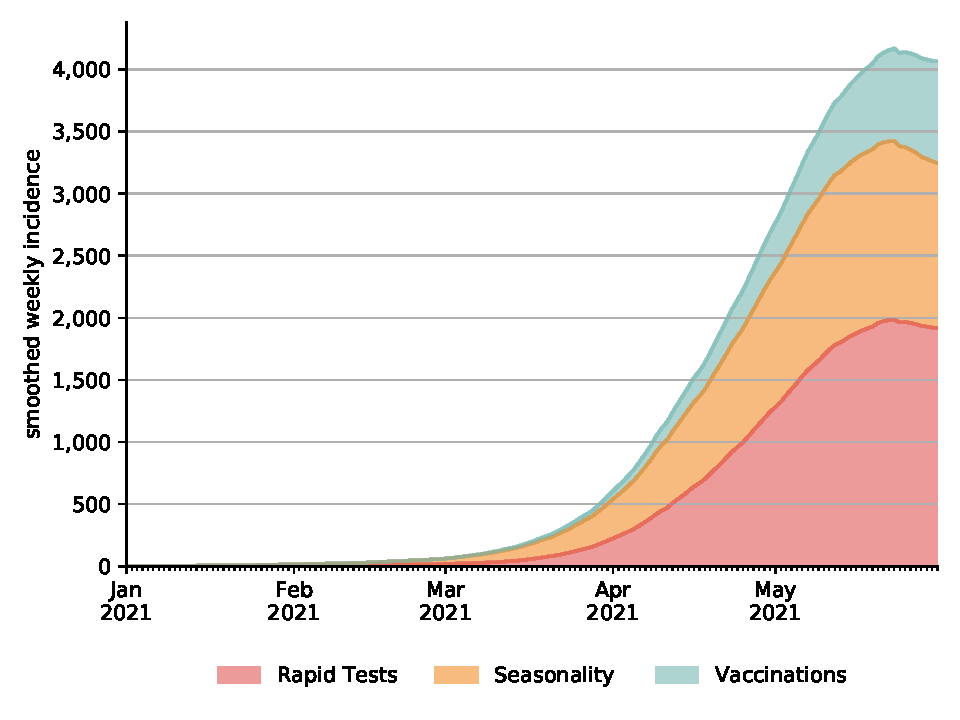
\includegraphics[width=\textwidth]{../figures/results/figures/full_decomposition_channels_area}
        % 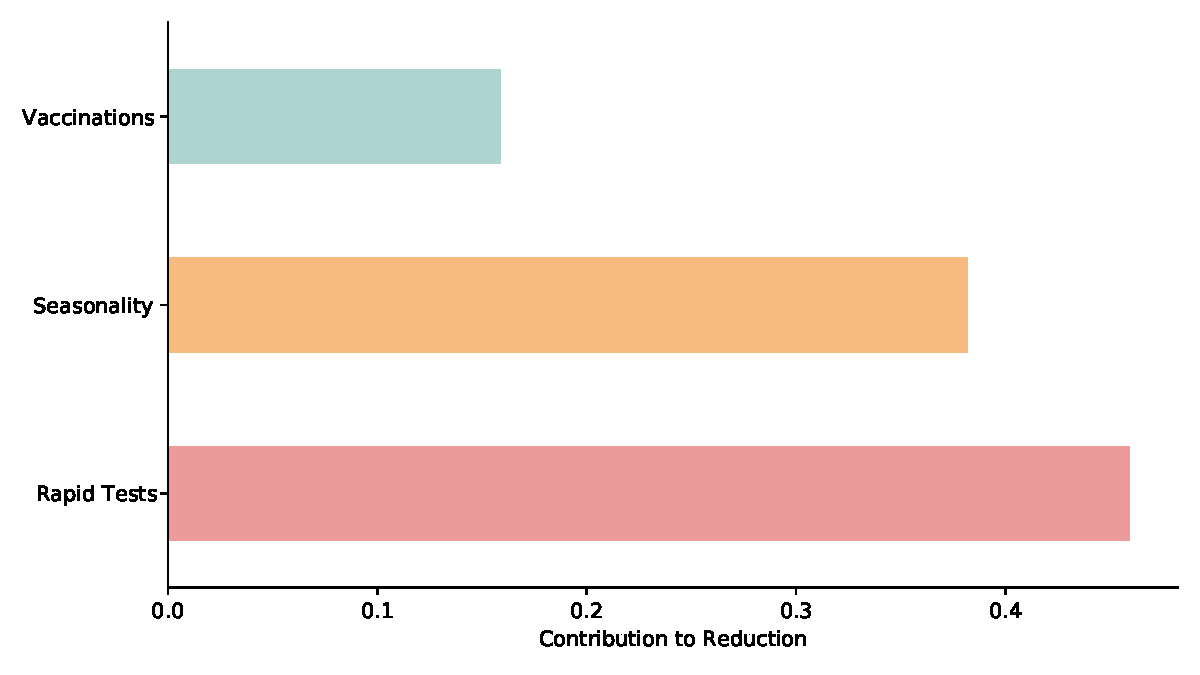
\includegraphics[width=\textwidth]{../figures/results/figures/full_decomposition_channels_bar}
        \caption{Decomposition of the difference between the scenario without any of the
            three factors and the main scenario in
            Figure~\ref{fig:2021_scenarios_newly_infected}.}
        \label{fig:2021_scenarios_decomposition}
    \end{subfigure}
    \hfill
    \begin{subfigure}[b]{0.475\textwidth}
        \centering
        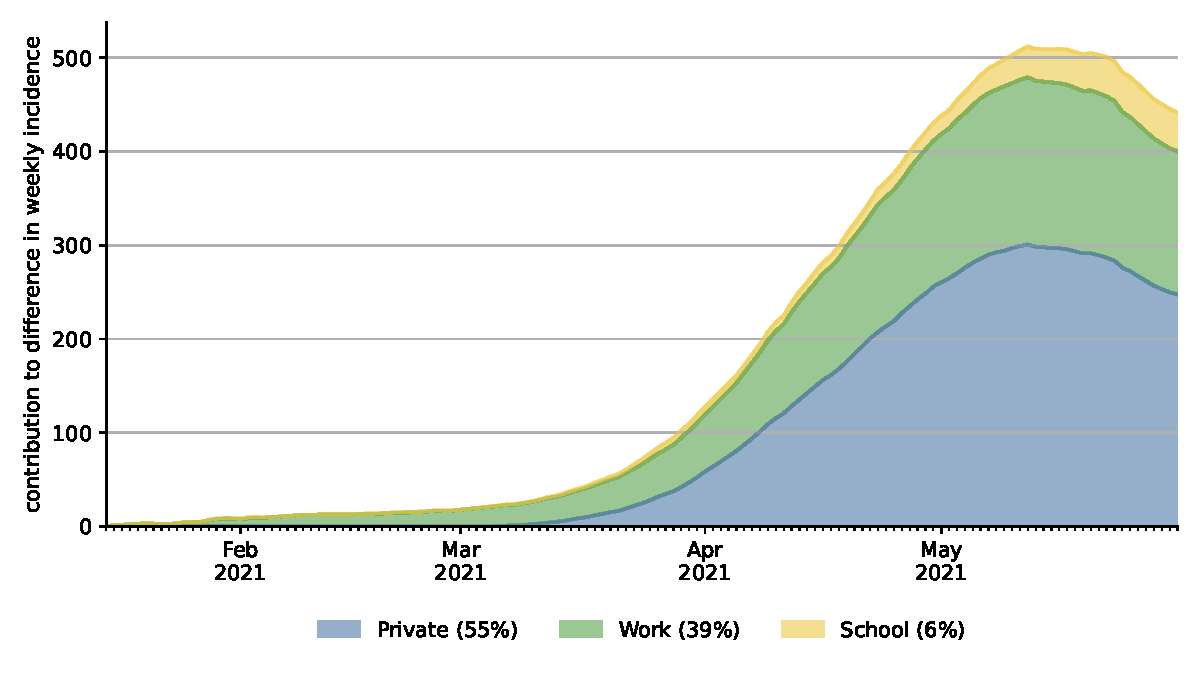
\includegraphics[width=\textwidth]{../figures/results/figures/full_decomposition_rapid_tests_area}
        % 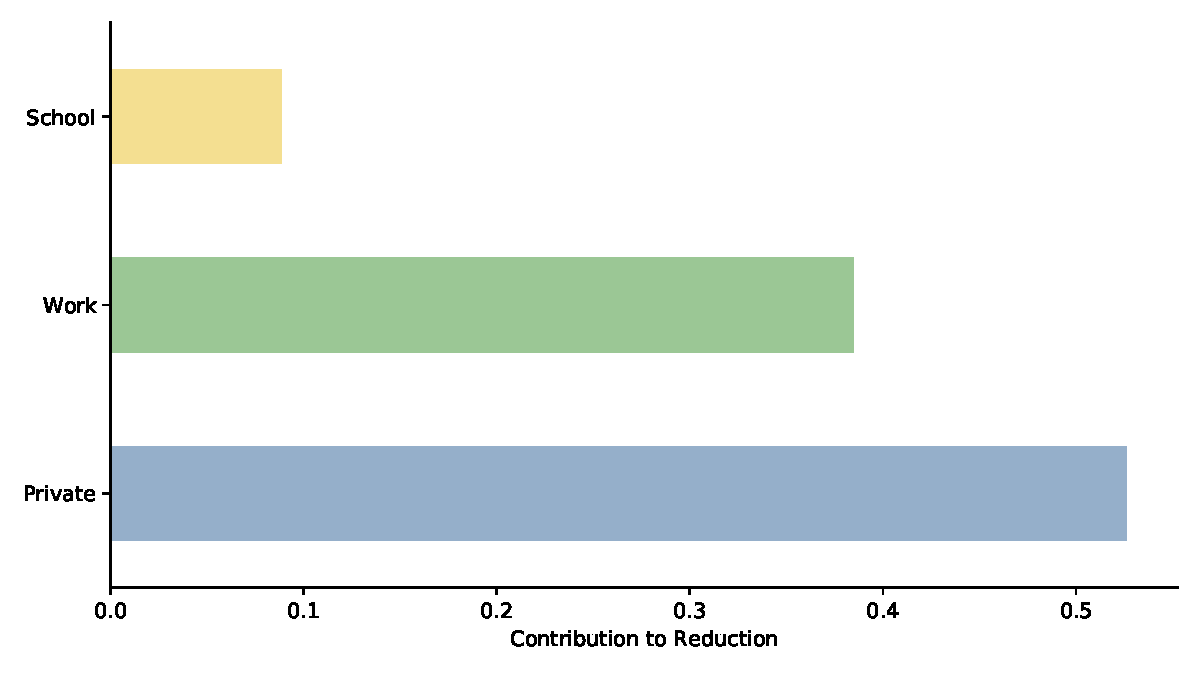
\includegraphics[width=\textwidth]{../figures/results/figures/full_decomposition_rapid_tests_bar}
        \caption{Decomposition of the difference between the scenario without rapid
            tests and the main scenario in Figure~\ref{fig:2021_scenarios_newly_infected}.}
        \label{fig:2021_scenarios_decomposition_tests}
    \end{subfigure}

    \caption{The effect of different interventions on recorded and actual infections}
    \label{fig:2021_scenarios_broad}

    \floatfoot{\noindent Note: All aggregates; See S.XXX for statistics by age group and
        by geographical region.

        The decomposition is based on Shapley values where the individual contribution
        of a channel is its average contribution over different sizes of coalitions
        (combinations with other channels). The individual contribution to a coalition
        is the difference between the effect size of the coalition with the particular
        channel and without.}
\end{figure}

Until mid-March, there is no visible difference between the different scenarios.
Seasonality hardly changes, and only few vaccinations or rapid tests were administered.
Even thereafter, the effect of the vaccination campaign is surprisingly small at first
sight. Whether considering recorded or total infections, the final level is always the
highest in case the vaccination campaign had been running in isolation (red lines). The
Shapley value decomposition shows that vaccinations contribute about
15\%\comment[id=HM]{check!} to the cumulative difference between scenarios. Reasons for
this are the slow start---it took until 24~March until 10\% of the population had
received their first vaccination, the 20\% mark was reached on April 19th ---and the
focus on older individuals. These groups contribute less to the spread of the disease
than others due to a lower number of contacts, see~\ref{fig:assortativity}. It is
important to note that the initial focus of the campaign was to prevent deaths and
severe disease; the case fatality was rate considerably lower during the third wave when
compared to the second (4.4\% between October and February and 1.4\% between March and
June). It is important to note that by the end of our study period, when first-dose
vaccination rates reached around 40\% of the population, the numbers of new cases would
have started to decline.

Seasonality has a large effect in slowing the spread of SARS-CoV-2. By May 31, both
observed and recorded cases would be reduced by a factor of four if only seasonality
mattered. However, in this period, cases would have kept on rising throughout, just at a
much lower pace. Nevertheless, we estimate it to be a quantitatively important factor
determining the evolution of the pandemic, explaining most of the early changes and
almost 40\% of the cumulative difference by the end of May.

The largest effect---almost one half when considering the decompositions---comes from
rapid testing. Here, it is crucial to differentiate between recorded cases and actual
cases. Additional testing means that infections become known which would otherwise
remain undetected. Figure~\ref{fig:2021_scenarios_recorded} shows that this means that
until late April, recorded cases are higher than in the scenario where none of the three
mechanisms is turned on. Compared to the scenario with vaccinations only, this point is
reached around mid-May and it would be June for the comparison with the seasonality-only
scenario. The effect on total cases, however, is visible immediately. Despite the fact
that only a small fraction of the population performed weekly rapid tests in
March\footnote{X\% in the model; 27\% of respondents to the COSMO study reported in
    early March that they \textit{ever} did a rapid test)}\comment[id=HM]{Put in}, new
infections on April 1 would be reduced by 53\% relative to the scenario without
vaccinations, rapid tests, or seasonality.

So why is rapid testing so effective? In order to shed more light on this question,
Figure~\ref{fig:2021_scenarios_decomposition_tests} decomposes the difference in the
scenario without rapid tests only (purple line in
Figure~\ref{fig:2021_scenarios_newly_infected}) and the main specification into the
three channels for rapid tests. Tests for pupils have the smallest effect, which is
largely explained by the relatively small number of students (XXM vs. YYM workers) and
the fact that schools did not operate at full capacity during our period of study.
Almost 40\% come from tests at the workplace. Despite the fact that we phase rapid tests
for private reasons are phased in only late, they make up for more than half of the total effect.

\comment[id=HM]{How many tests are actually performed along each of the three dimensions? Could this be a quantity story rather than the directed testing story I am making up here as wishful thinking?}

The reason lies in the fact that a substantial share of these tests is driven by an
elevated probability to carry the virus, i.e., showing symptoms of CoViD-19 or following
up on a positive test of a household member. The latter is essentially a form of contact
tracing, which has been shown to be very effective.\comment[id=HM]{cite Priesemann
paper, others?} This is also the reason for why the number of tests performed fall at
the very end of our study period. Falling infection rates mean that there are fewer
events triggering private test demand.
\comment[id=HM]{Positive rates along the three channels might be nice here, if previous comment is not a quant story}
\comment[id=HM]{I think there is a story in here about risk conditional on past exposure vs. prospective risk in gatherings, but it is too late to work through it. We might just want to calculate the probabilities.}

Two of the most contentious NPIs concern schools and mandates to work from home. In many
countries, schools switched to remote instruction during the first wave, so did Germany.
After the summer break, they were operating at full capacity with increased hygiene
measures, before being closed again from mid-December on. Some states started opening
them gradually in late February, but usual operaton was not back until the beginning of
June. In light of the large negative effects school closures have on children and
parents\comment[id=HM]{need to cite a couple of poor learning outcomes / mental health
papers. There must be well-published ones}---and in particular on those with low
socio-economic status---

Effects:
\begin{itemize}
    \item Schools were essentially closed
    \item What are the different $R_t$-values? In no-test scenario and $R_t>1$, might be
          worth chopping off 0.05 or whatever that might be?
    \item With tests it is really hard to make a case for that
\end{itemize}

Alternative:
\begin{itemize}
    \item Germany quite lenient on home office relative to other countries (employer had
          to allow)
    \item Testing: Rapid tests are cheap (less than 1\euro), just a nuisance.
\end{itemize}

Results
\begin{itemize}
    \item Advantage of testing in both cases: Recurrent. Small cost relative to other
          stuff. Certain publicness.
    \item Mandatory tests: Screening effect for hard-to-reach populations (do not
          consider in this paper, also due to poor data in DE)
\end{itemize}


\begin{figure}[!tp]
    \centering

    \begin{subfigure}[b]{0.475\textwidth}
        \centering
        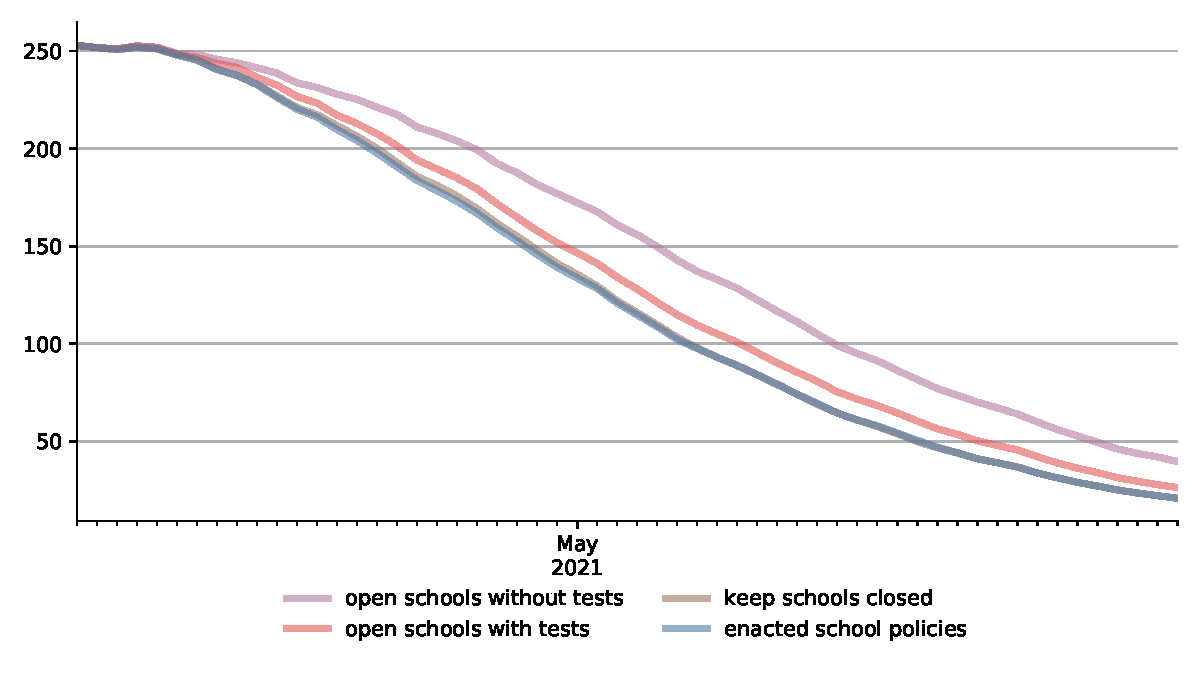
\includegraphics[width=0.9 \textwidth]{../figures/results/figures/scenario_comparisons/school_scenarios/full_newly_infected}
        \caption{{Effects of different schooling scenarios after Easter}}
        \label{fig:schooling_scenarios_easter}
    \end{subfigure}
    \hfill
    \begin{subfigure}[b]{0.475\textwidth}
        \centering
        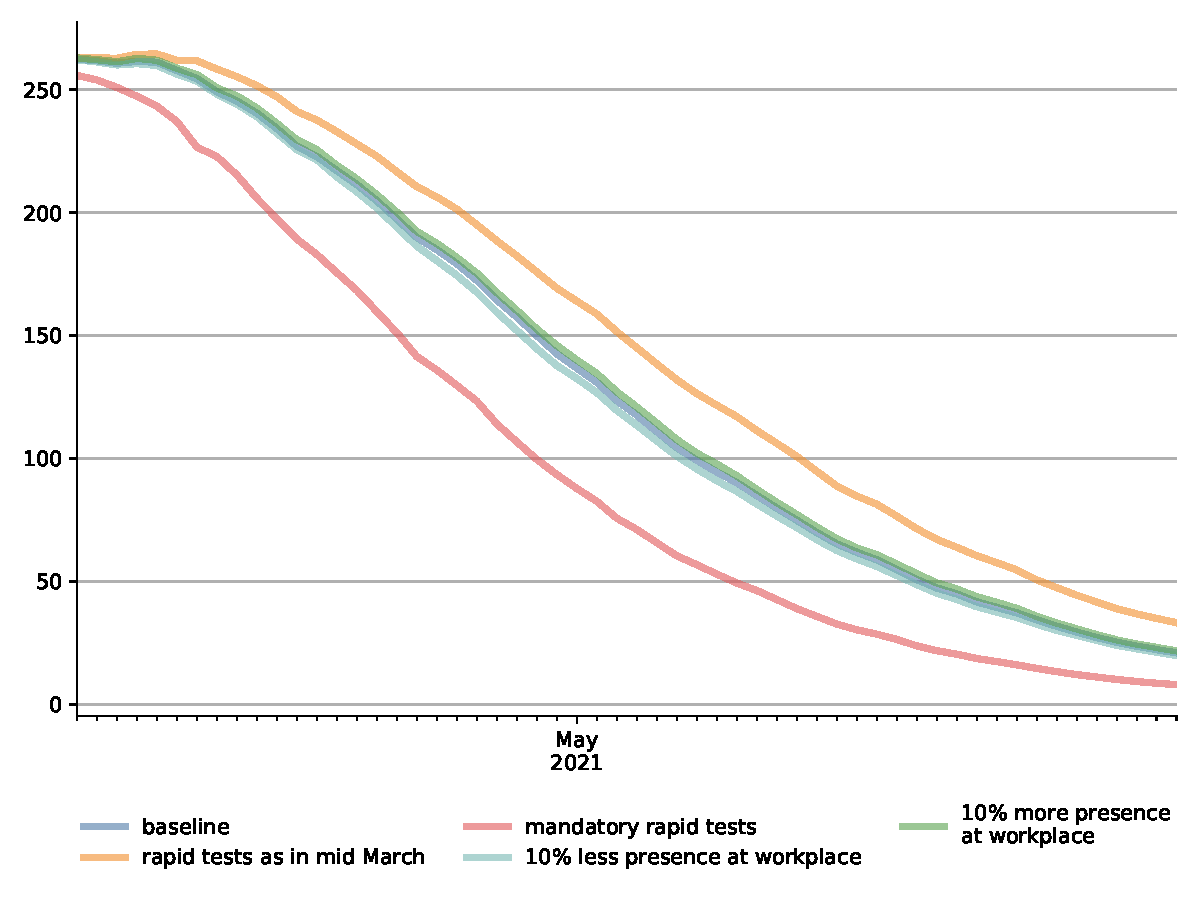
\includegraphics[width=0.9 \textwidth]{../figures/results/figures/scenario_comparisons/new_work_scenarios/full_newly_infected}
        \caption{{Effects of different work scenarios after Easter}}
        \label{fig:to_be_determined}
    \end{subfigure}
    \vskip3ex

    \caption{Effects of different scenarios for schooling and working from home}
    \label{fig:interventions_school}

    \floatfoot{\noindent Note: All aggregates; See S.XXX for statistics by age group and
        by geographical region.}

\end{figure}
